%!TEX root =  main.tex

\lectureheader{162}{Calculus II}{Inverse trigonometric functions}{\textit{Thomas' Calculus} \textsection 7.6}

\begin{remark}
The trigonometric functions are periodic, and so they can't have inverses.
So, we do the best that we can. 
As with the square and square-root, we invert a preferred ``slice" of each.
\end{remark}

\begin{example}
For each of the six trigonometric functions, identify an interval of the domain for which the function is one-to-one and onto its full range.
\end{example}

\newpage

\begin{definition}
The six ``inverse" trigonometric functions are defined by the rules:
\begin{enumerate}
\item $y=\arcsin x \iff \sin y = x$ and $y\in [-\pi/2, \pi/2]$.
\item $y = \arccos x \iff \cos y = x$ and $y\in [0,\pi]$.
\item $y = \arctan x \iff \tan y = x$ and $y\in (-\pi/2, \pi/2)$.
\item $y=\arccsc x \iff \csc y = x$ and $y\in [-\pi/2, 0)\cup (0, \pi/2]$.
\item $y = \arcsec x \iff \sec y = x$ and $y\in [0, \pi/2)\cup (\pi/2, \pi]$.
\item $y = \arccot x \iff \cot y = x$ and $y\in (0,\pi)$.
\end{enumerate}
\end{definition}
\begin{remark}\,
\begin{itemize}
\item We call them inverse trigonometric functions, but that's really a lie!  They're impostors!
\item Even though I don't like it, we will also use the alternative notation $\sin^{-1} x = \arcsin x$, $\cos^{-1} x = \arccos x$, etc.
\end{itemize}
\end{remark}

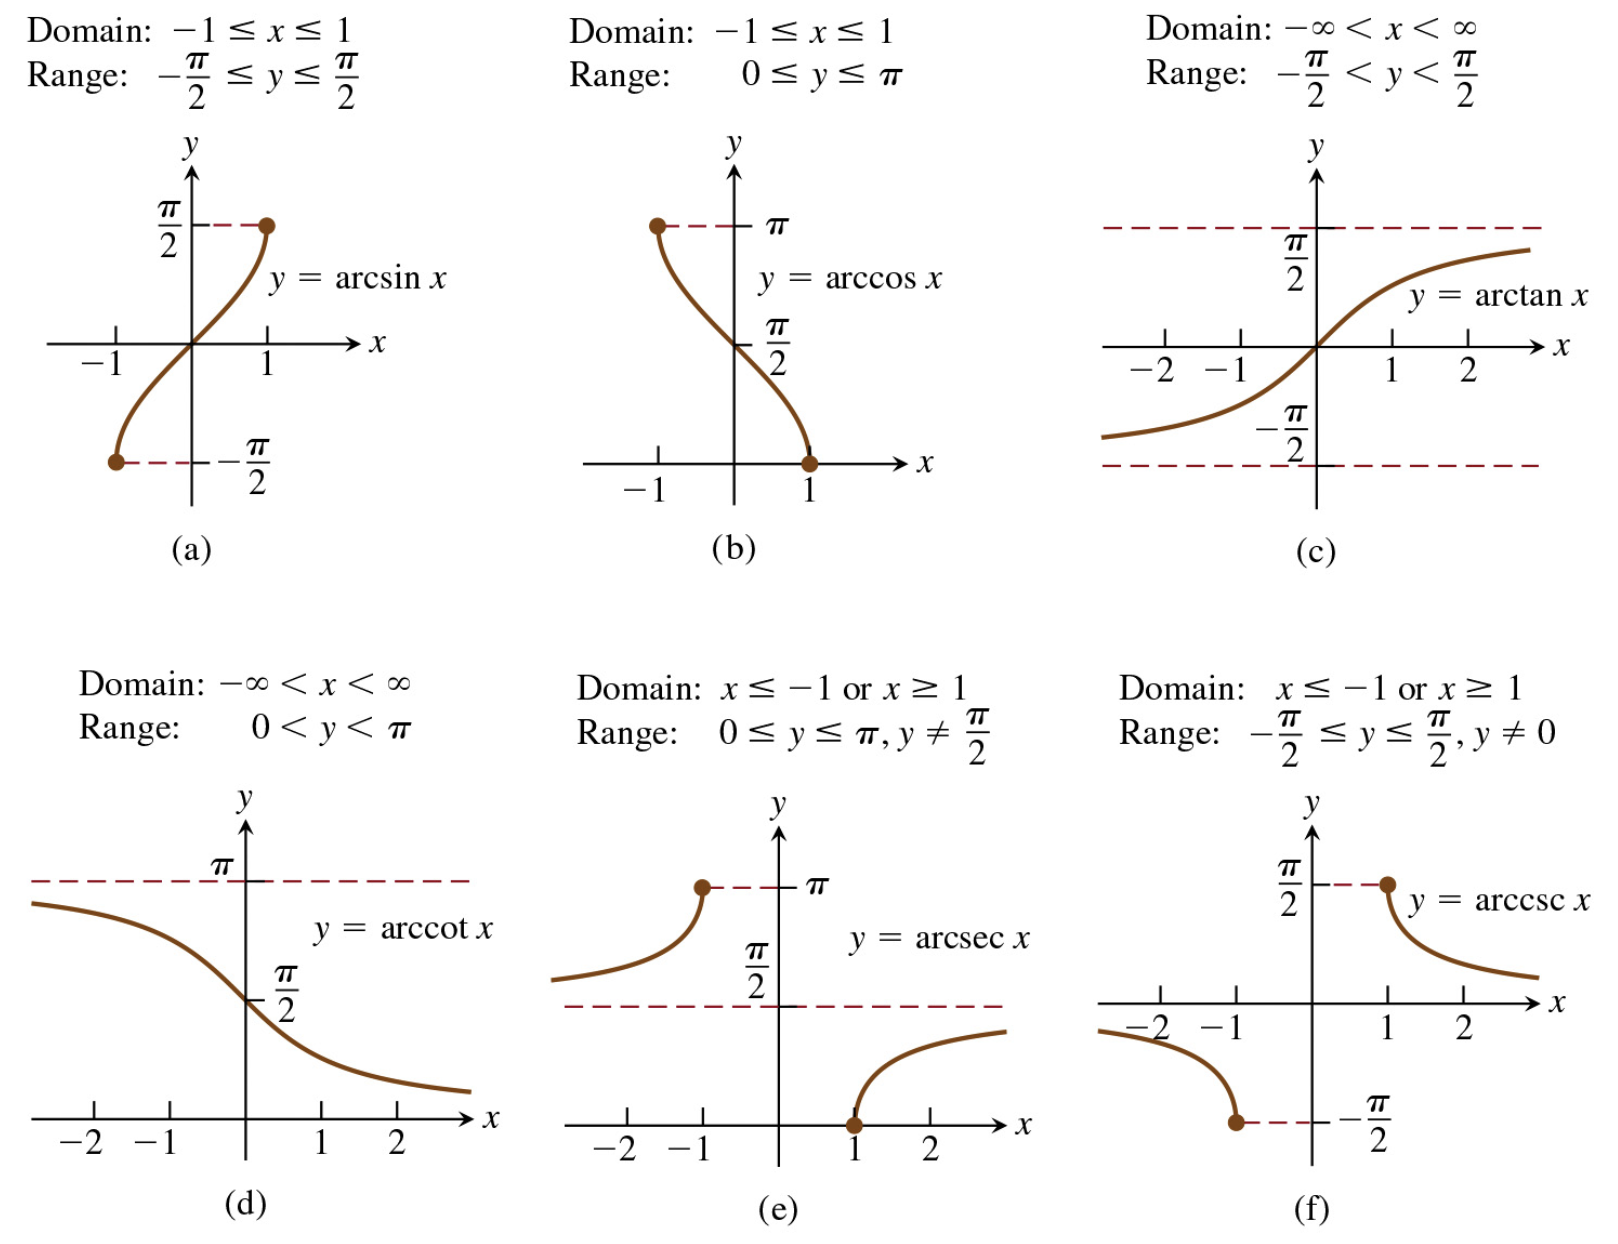
\includegraphics[width=6.5in]{img/inverse_trig_graphs}

\newpage

\begin{example}
Evaluate the following.
\begin{enumerate}
\item $\arcsin(\sqrt 3/2)$
\vfill
\item $\arcsin(-\sqrt 2/2)$
\vfill
\item $\arccos(-1/2)$
\vfill
\item $\arcsin(\sin(5\pi/8))$
\vfill
\end{enumerate}
\end{example}

\newpage

\begin{theorem}
\begin{align}
\frac{\dee}{\dee x}\arcsin x &= \frac{1}{\sqrt{1-x^2}}\quad (|x|<1),\\
\frac{\dee}{\dee x}\arccos x &= \frac{-1}{\sqrt{1-x^2}}\quad (|x|<1),\\
\frac{\dee}{\dee x}\arctan x &= \frac{1}{1+x^2},\\
\frac{\dee}{\dee x}\arccsc x &= \frac{-1}{|x|\sqrt{x^2-1}}\quad (|x|>1),\\
\frac{\dee}{\dee x}\arcsec x &= \frac{1}{|x|\sqrt{x^2-1}}\quad (|x|>1),\\
\frac{\dee}{\dee x}\arccot x &= \frac{-1}{1+x^2}.
\end{align}
\end{theorem}

\begin{proof}\,

\vspace{3.5in}
\end{proof}

\begin{corollary}
\begin{align}
\int \frac{\dee x}{\sqrt{1-x^2}} &= \arcsin x + C\quad (|x|<1),\\
\int \frac{\dee x}{1+x^2} &= \arctan x + C,\\
\int \frac{\dee x}{|x|\sqrt{x^2-1}} &= \arcsec|x| + C\quad (|x|>1).
\end{align}
\end{corollary}

\newpage

\begin{example}
Compute $\dee y/\dee x$ if $y=\arcsin x^2$.
\end{example}
\vfill

\begin{example}
Evaluate the following.
\begin{enumerate}
\item $\DS\int_{\sqrt 2/2}^{\sqrt 3/2}\frac{\dee x}{\sqrt{1-x^2}}$
\vfill
\item $\DS\int\frac{\dee x}{\sqrt{3-4x^2}}$
\vfill
\end{enumerate}
\end{example}

\newpage

\begin{example}
Compute the following integrals.
\begin{enumerate}
\item $\DS\int\frac{\dee x}{\sqrt{\E^{2x}-6}}$
\vfill
\item $\DS\int\frac{\dee x}{\sqrt{4x-x^2}}$
\vfill
\item $\DS\int\frac{\dee x}{4x^2+4x+2}$
\vfill
\end{enumerate}
\end{example}

